\documentclass[12pt, french]{article}

\usepackage{fancyhdr, fancybox, lastpage, makecell}
\usepackage[most]{tcolorbox}
\usepackage[a4paper, margin={0.3in, .75in}]{geometry}
\usepackage{wrapfig}
\pagestyle{fancy}
\renewcommand\headrulewidth{1pt}
\renewcommand\footrulewidth{1pt}
\fancyhf{}
\rhead{ \em{Zakaria Haouzan}}
\lhead[C]{\em{2ème année baccalauréat SM}}
\chead[C]{}
\rfoot[C]{}
\lfoot[R]{ \emph{TD-Modulation (AM)}}
\cfoot[]{\em{Page \thepage / \pageref{LastPage}}}


\newtcolorbox{Box2}[2][
enhanced,
breakable
]{
                lower separated=false,
                colback=white,
colframe=white!20!black,fonttitle=\bfseries,
colbacktitle=white!30!gray,
coltitle=black,
enhanced,
attach boxed title to top left={yshift=-0.1in,xshift=0.15in},
title=#2,#1}


\begin{document}
\begin{center}
   \shadowbox {\bf{Production d'ondes électromagnétiques et
communication.}}
\end{center}

\vspace{-0.2cm}
%%_________________________Exercice ! :"_________________________Exercice
%   \begin{center}
	   %\vspace{-0.6cm}
	%\includegraphics[width=0.6\textwidth ]{./img/Exercice01.png}
  %\end{center}



\begin{Box2}{\textbf{Exercice 1 :Transmission des signaux sonores} }
\begin{wrapfigure}{r}{0.22\textwidth}
  \begin{center}
	  \vspace{-0.6cm}
	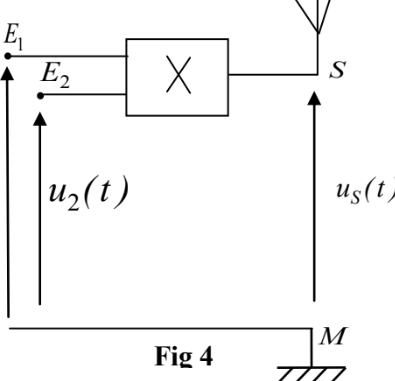
\includegraphics[width=0.22\textwidth]{./fig00M.png}
  \end{center}
\end{wrapfigure}

Les ondes sonores audibles ont une faible fréquence, leur transmission à des longues distances nécessite qu'elles soient modulante à une onde électromagnétique de haute fréquence.

Cet exercice vise à étudier la modulation et la demodulation.

\begin{wrapfigure}{r}{0.4\textwidth}
  \begin{center}
	  \vspace{-5.5cm}
	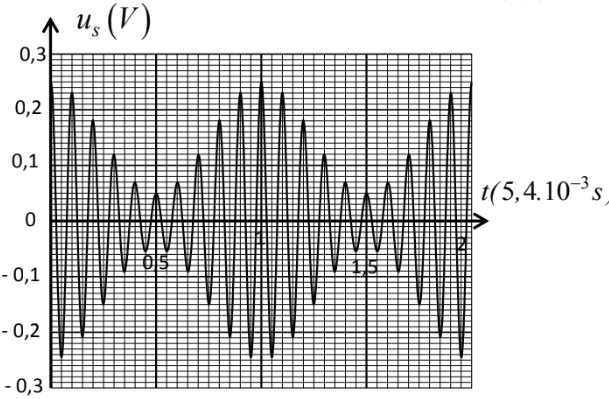
\includegraphics[width=0.44\textwidth]{./fig01M.png}
  \end{center}
\end{wrapfigure}

\subsection*{1 - Modulation}
On considère le montage représenté dans la figure 4 :
\begin{itemize}
    \item Le générateur (GBF\textsubscript{1}) applique à l'entrée E\textsubscript{1} de la composante électronique X une tension sinusoïdale :
    \[u_1(t) = P_m\cos\left(\frac{2\pi}{T_p}t\right)\]
    
    \item Le générateur (GBF\textsubscript{2}) applique à l'entrée E\textsubscript{2} de la composante électronique X une tension sinusoïdale :
    \[u_2(t) = U_0 + S(t)\]
    avec U\textsubscript{0} la composante continue de la tension et
    \[S(t) = S_m\cos\left(\frac{2\pi}{T_s}t\right)\]
    la tension correspondante à l'onde qu'on désire\\ transmettre.
\end{itemize}

On visualise sur l'écran d'un oscilloscope la tension de sortie \[u_s(t) = k\cdot u_1(t)\cdot u_2(t)\] avec k constante positive caractérisant la composante X, fig 5.


\begin{enumerate}
  \item Montrer que l'expression de la tension u\textsubscript{s}(t) s'écrit sous la forme :
\[u_s(t) = A\left(1 + m\cos\left(\frac{2\pi}{T_s}t\right)\right)\cos\left(\frac{2\pi}{T_p}t\right)\]
et préciser l'expression de A et celle de m.

  
\item Calculer la valeur de m et déduire la qualité de la modulation.

\end{enumerate}
\subsection*{2 - Démodulation}
La figure 6 représente le montage utilisé dans un dispositif de réception constitué de trois parties.
  \begin{center}
	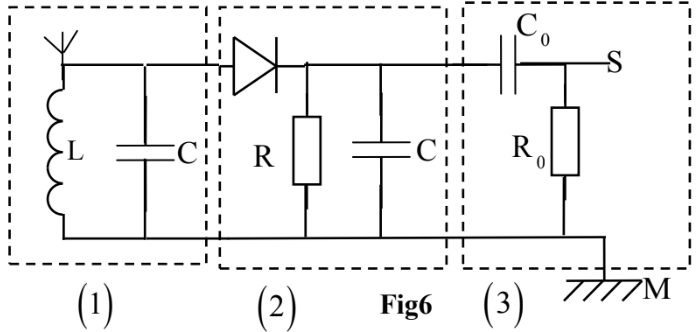
\includegraphics[width=0.44\textwidth]{./fig02M}
  \end{center}

\begin{enumerate}
  
  \item Préciser le rôle de la partie 3 dans ce montage.

  \item Déterminer la valeur du produit L·C pour que la sélection de l'onde soit bonne.

  \item Montrer que l'intervalle auquel doit appartenir la valeur de la résistance R pour une bonne détection de l'enveloppe de la tension modulante dans ce montage est :
\[\frac{2\pi}{T_p} \ll \frac{1}{RC} \ll \frac{2\pi}{T_s}\]

\item Calculer les bornes de cet intervalle sachant que L = 1,5 mH.

\end{enumerate}

%\vspace{1cm}
\end{Box2}

\begin{Box2}{\textbf{Exercice 2 : Modulation d’amplitude d’un signal sinusoïdal}}


\begin{wrapfigure}{r}{0.22\textwidth}
  \begin{center}
	  \vspace{-0.5cm}
	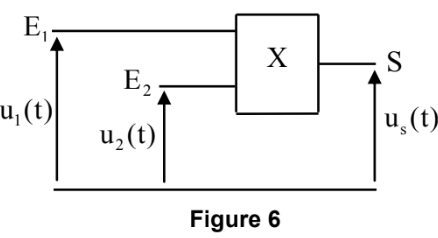
\includegraphics[width=0.22\textwidth]{./fig03M.png}
  \end{center}
\end{wrapfigure}


Afin d'obtenir un signal modulé en amplitude, on utilise un circuit intégré multiplieur X (figure 6).

On applique à l'entrée :
\begin{itemize}
    \item $E_1$ : la tension $u_1(t) = s(t) + U_0$ avec $s(t) = S_m\cos(2\pi f_s t)$ représentant le signal informatif et $U_0$ une composante continue de la tension.
    \item $E_2$ : une tension sinusoïdale représentant la porteuse $u_2(t) $=$ U_m\cos(2\pi F_p t)$
\end{itemize}

La tension de sortie $u_s(t)$ obtenue est $u_s(t) = k\cdot u_1(t)\cdot u_2(t)$ ; $k$ est une constante qui dépend du circuit intégré X.

\textbf{Rappel :} $\cos(a)\cos(b) = \frac{1}{2}[\cos(a-b) + \cos(a+b)]$

  \begin{center}
	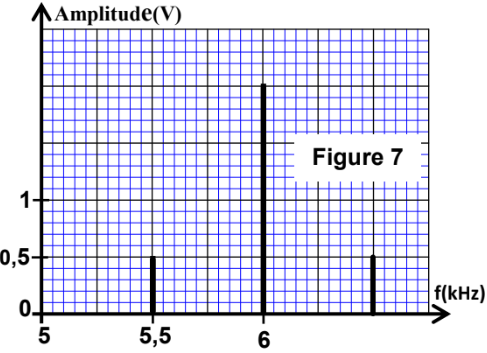
\includegraphics[width=0.4\textwidth]{./fig04M.png}
  \end{center}

\begin{enumerate}
    \item Montrer que $u_s(t)$ s'écrit sous la forme :
    $$u_s(t) = \frac{A\cdot m}{2}\cos(2\pi f_s t) + A\cos(2\pi f_p t) + \frac{A\cdot m}{2}\cos(2\pi f_3 t)$$
    où $m$ est le taux de modulation et $A$ une constante.

    \item La figure 7 représente le spectre de fréquences formé de trois raies de la tension modulée $u_s(t)$. Déterminer $m$ et la fréquence $f_s$. La modulation est-elle bonne ?
    \item Pour une bonne réception du signal modulé, on utilise un circuit bouchon (circuit d'accord) formé d'une bobine d'inductance $L_0 = 60mH$ et de résistance négligeable et de deux condensateurs, montés en série, de capacité $C = 10\mu F$ et $C_0$. Déterminer la valeur de $C_0$.
\end{enumerate}
\end{Box2}

%\vspace{2cm}
%\begin{center}
   %\Large{ \em{Exercices Supplémentaires}}
%\end{center}


%\vspace{-0.7cm}
%%_________________________Exercice 5 : _________________________Exercice
%\begin{Box2}{Exercice 5 :Les ondes sonores }
%4
%\end{Box2}
%%_________________________Exercice 6 : _________________________Exercice
%\begin{Box2}{Exercice 6 : échographie}
%6
%\end{Box2}

\end{document}
